\documentclass[11pt]{article}

\usepackage{fontspec}
\usepackage{amsmath}
\usepackage{graphicx}
\usepackage{enumitem}
\usepackage{listings}
\usepackage{xcolor}
\usepackage{float}

\newcommand{\picturewidth}{7cm}

\setmainfont{DejaVu Serif}

\definecolor{codegreen}{rgb}{0,0.6,0}
\definecolor{codegray}{rgb}{0.5,0.5,0.5}
\definecolor{codepurple}{rgb}{0.58,0,0.82}
\definecolor{backcolour}{rgb}{0.95,0.95,0.92}

\lstdefinestyle{mystyle}{
  backgroundcolor=\color{backcolour},
  commentstyle=\color{codegreen},
  keywordstyle=\color{magenta},
  numberstyle=\tiny\color{codegray},
  stringstyle=\color{codepurple},
  basicstyle=\ttfamily\footnotesize,
  breakatwhitespace=false,         
  breaklines=true,                 
  captionpos=b,                    
  keepspaces=true,                                   
  showspaces=false,                
  showstringspaces=false,
  showtabs=false,                  
  tabsize=2
}
\lstset{style=mystyle}

\begin{document}

\begin{center}
    {\huge УЧЕБЕН ПРОЕКТ} \\
    по \\
    {\huge „Диференциални уравнения и приложения“} \\
    спец. Софтуерно инженерство, 2 курс, летен семестър,  \\
    учебна година 2023/2024 \\
    Тема СИ2024-УП-4.11. \\
    \vspace{0.5cm}
\end{center}

\begin{flushright}
    \begin{tabular}{rl}
        Изготвил: & Ивайло Ангелов Андреев \\
        Ф. №:     & 4MI0600186 \\
        Група:    & 4 \\
    \end{tabular}
\end{flushright}

\begin{flushleft}
    \begin{tabular}{rl}
        & 08.06.2024г. \\
        & София \\
    \end{tabular}
\end{flushleft}

\newpage
\tableofcontents
\newpage

\section{ТЕМА (ЗАДАНИЕ) НА ПРОЕКТА}
\begin{flushleft}
    Дадена е задачата на Коши за уравнението на хармоничния осцилатор:
\end{flushleft}
$$
\begin{cases}
    y'' + ky' + 5y = a \cos(\omega_0 \, t) \\
    y(0) = -1 \\
    y'(0) = 1 \\
\end{cases}
$$
\begin{flushleft}
    Дадена е задачата на Коши за уравнението на хармоничния осцилатор:
    \begin{enumerate}[label=\arabic*.]
        \item (4 т.) Решете символно задачата с MATLAB дадената задача при $k = 0.3$ и $a = 0$.
        Начертайте графиката на намереното решение в интервала $[0,50]$.
        \item (3 т.) При $k = 0$ и $a = 2$ изберете подходяща стойност на честотата $\omega_0$ на външната сила така, че
        да демонстрирате явлението резонанс.
        \item (3 т.) При $k = 0$ и $a = 2$ изберете подходяща стойност на честотата $\omega_0$ на външната сила така, че
        да демонстрирате явлението биене.
        \item (10 т.) Решете символно с MATLAB получените задачи в подточки (2) и (3) и начертайте графиките
        на решенията им в същия интервал както в подточка (1). Разположете всички графики една под друга.
    \end{enumerate}
\end{flushleft}

\newpage

\section{РЕШЕНИЕ НА ЗАДАЧАТА}

\subsection{Теоретична част}
\begin{flushleft}
    Нека разгледаме уравнението на хармоничния осцилатор в общия случай. 
    $$
    \begin{cases}
        y'' + ky' + 5y = f(t) \\
        y(0) = \eta_0 \\
        y'(0) = \nu_0 \\
    \end{cases}
    $$
    $k$ - коефициент на загуба на енергия \\
    $\omega > 0$ - собствена честота на системата \\
    $\eta_0$ - начално положение \\
    $\nu_0$ - начална скорост \\
    $f(t)$ - външна сила, която действа на системата \\
    За $f(x) = a \cos(\omega_0 \, t)$ имаме, че $\omega_0$ е честотата на външната сила. \\
    \vspace{0.35cm}

    За подточка (1) имаме следното:
    $$y'' + 0.3y' + 5y = 0$$
    Това уравнение демонстрира явлението триене. \\
    \vspace{0.25cm}
    Идея за решаване аналитично: \\
    \vspace{0.20cm}
    Това е хомогенно линейно ОДУ от втори ред. \\
    Представяме характеристичния полином на уравнението:
    $$P(\lambda) = \lambda^2 + 0.3\lambda + 5 = 0$$
    $$10\lambda^2 + 3\lambda + 50 = 0$$
    $$\lambda_{1,2} = \dfrac{-3 \pm \sqrt{3^2 - 4 \times 10 \times 50}}{2 \times 10}$$
    $$\lambda_{1,2} = \dfrac{-3}{20} \pm i \dfrac{\sqrt{1991}}{20}$$
    Оттук представяме фундаменталната система решения:
    $$
    \text{ФСР} = \left\{e^{-\frac{3}{20}t}\cos\left(\dfrac{\sqrt{1991}}{20}t\right), \,\,
        e^{-\frac{3}{20}t}\sin\left(\dfrac{\sqrt{1991}}{20}t\right)\right\}
    $$
    Така обшия вид на хомогенното уравнение е: \\
    $$
    y = C_1 e^{-\frac{3}{20}t}\cos\left(\dfrac{\sqrt{1991}}{20}t\right) +
        C_2 e^{-\frac{3}{20}t}\sin\left(\dfrac{\sqrt{1991}}{20}t\right)
    $$
    Можем да намерим точното уравнение, решение на задачата на Коши, като заместим с началните условия от задачата на Коши. \\

    \vspace{0.35cm}
    За подточки (2) и (3) имаме следното:
    $$y'' + 5y = 2 \cos(\omega_0 \, t)$$
    Имаме следното:
    $$
    \begin{cases}
    \omega^2 = 5 \\
    \omega > 0 \\
    \end{cases}
    $$
    Откъдето $\omega = \sqrt{5}$ \\

    \vspace{0.15cm}
    {\huge Резонанс \\}
    Резпнанс се демонстрира, когато честотата на външната сила е равна на собствената честота на системата.
    А именно:
    $$\omega_0 = \omega = \sqrt{5}$$

    \vspace{0.15cm}
    {\huge Биене \\}
    Биене се демонстрира, когато честотата на външната сила е близка до собствената честота на системата.
    А именно:
    $$\omega_0 = \omega + \epsilon = \sqrt{5} + \epsilon; \quad \epsilon > 0$$

    \noindent
    \hrule height 0.1pt
    \vskip 0.2cm

    Идея за решаване аналитично на:
    $$y'' + 5y = 2 \cos(\omega_0 \, t)$$
    \vspace{0.20cm}
    Това е нехомогенно линейно ОДУ от втори ред. \\
    Първо ще намерим общото решение на хомогенното уравнение. \\
    Представяме характеристичния полином на уравнението: \\
    $$P(\lambda) = \lambda^2 + 5 = 0$$
    $$\lambda^2 = -5$$
    $$\lambda_{1,2} = \pm i \sqrt{5}$$
    Оттук представяме фундаменталната система решения:
    $$\text{ФСР} = \{\cos(\sqrt{5}t), \,\, \sin(\sqrt{5}t)\}$$
    Така обшoто решение на хомогенното уравнение е: \\
    $$y_0 = C_1 \cos(\sqrt{5}t) + C_2 \sin(\sqrt{5}t)$$

    Търсим частно решение на нехомогенно уравнение:
    $$y'' + 5y = 2 \cos(\omega_0 t)$$
    $$e^{i\,\omega_0\,t} = \cos(\omega_0 t) + i\sin(\omega_0 t)$$
    Откъдето $\,\cos(\omega_0 t) = \text{Re}(e^{i \omega_0 t})$
    Ще намеим частно решение на уравнението:
    $$y'' + 5y = 2 e^{i\,\omega_0 t}$$
    $2 e^{i \omega_0 t}$ е квазиполиноим от вида $P^0 e^{\alpha t}$,
        където $P^0 = 2$ е полином от нулева степен и $\alpha = i\omega_0$. \\
    Така частното решение на уравнението $y_1$ има вида:
    $$y_1 = t^s Q^0 e^{\alpha t},$$
    където $\alpha = i\omega_0$, $s$ е показва, че $\alpha$ е $s$-кратен корен на характеристичния полином $P(\lambda)$,
        а $Q^0(t) = at^0 = a$ е произволен полином от нулева степен.

    {\LARGE I-ви случай: при резонанс}
    $$\omega_0 = \sqrt{5}$$
    $$\alpha = i\sqrt{5} \in \{\lambda_i\} \quad i \in \{1, 2\}$$
    $$y_1 = t^1 a e^{i \omega_0 t}$$
    $$y_1 = ate^{i\sqrt{5} t}$$
    $$y_1'' = i2a\sqrt{5}e^{i\sqrt{5}t} - 5ate^{i\sqrt{5}t}$$

    С $y''$ и $y$ замесваме в уравнението $y'' + 5y = 2 e^{i \omega_0 t}$.

    $$i2a\sqrt{5}e^{i\sqrt{5}t} - 5ate^{i\sqrt{5}t} + 5ate^{i\sqrt{5} t} = 2e^{i\sqrt{5}t}$$
    $$i2a\sqrt{5} - 5at + 5at = 2$$
    $$i2a\sqrt{5} = 2$$
    $$ia\sqrt{5} = 1$$
    $$a = \dfrac{1}{i\sqrt{5}}$$
    $$a = -\dfrac{i\sqrt{5}}{5}$$
    
    Заместваме в $y_1$ с намерената стойност за $a$. \\

    $$y_1 = -i\dfrac{\sqrt{5}}{5}te^{i\sqrt{5} t}$$
    $$y_1 = -i\dfrac{\sqrt{5}}{5}t[\cos(\sqrt{5}t) + i\sin(\sqrt{5}t)]$$
    $$y_1 = -\dfrac{\sqrt{5}}{5}t[i\cos(\sqrt{5}t) - \sin(\sqrt{5}t)]$$
    $$y_1 = \dfrac{\sqrt{5}}{5}t\sin(\sqrt{5}t) - i\dfrac{\sqrt{5}}{5}t\cos(\sqrt{5}t)$$
    $$\text{Re}(y_1) = \dfrac{\sqrt{5}}{5}t\sin(\sqrt{5}t)$$

    Общото решение на нехомогенното уравнение $y'' + 5y = 2 \cos(\omega_0 \, t)$ е:

    $$y = y_0 + \text{Re}(y_1) = C_1 \cos(\sqrt{5}t) + C_2 \sin(\sqrt{5}t) + \dfrac{\sqrt{5}}{5}t\sin(\sqrt{5}t)$$

    Можем да намерим точното уравнение, решение на задачата на Коши, като заместим с началните условия от задачата на Коши. \\
    \vspace{0.2cm}

    {\LARGE II-ви случай: при биене}
    $$\omega_0 = \sqrt{5} + \epsilon \ne \sqrt{5} \quad \epsilon > 0$$
    $$\alpha \notin \{\lambda_i\} \quad i \in \{1, 2\}$$
    $$y_1 = t^0 a e^{i \omega_0 t}$$
    $$y_1 = ae^{i\omega_0 t} $$
    $$y_1'' = -a\omega_0^2e^{i\omega_0t}$$

    С $y''$ и $y$ замесваме в уравнението $y'' + 5y = 2 e^{i \omega_0 t}$.

    $$-a\omega_0^2e^{i\omega_0t} + 5ae^{i\omega_0 t} = 2e^{i\omega_0 t}$$
    $$-a\omega_0^2 + 5a = 2$$
    $$a = \dfrac{2}{5 - \omega_0^2}$$

    Заместваме в $y_1$ с намерената стойност за $a$. \\

    $$y_1 = \dfrac{2}{5 - \omega_0^2}e^{i\omega_0 t}$$
    $$y_1 = \dfrac{2}{5 - \omega_0^2}(\cos(\omega_0 t) + i\sin(\omega_0 t))$$
    $$y_1 = \dfrac{2}{5 - \omega_0^2}\cos(\omega_0 t) + i\dfrac{2}{5 - \omega_0^2}\sin(\omega_0 t)$$
    $$\text{Re}(y_1) = \dfrac{2}{5 - \omega_0^2}\cos(\omega_0 t)$$

    Общото решение на нехомогенното уравнение $y'' + 5y = 2 \cos(\omega_0 \, t)$ е:

    $$y = y_0 + \text{Re}(y_1) = C_1 \cos(\sqrt{5}t) + C_2 \sin(\sqrt{5}t) + \dfrac{2}{5 - \omega_0^2}\cos(\omega_0 t)$$

    Можем да намерим точното уравнение, решение на задачата на Коши, като заместим с началните условия от задачата на Коши. \\
\end{flushleft}

\newpage

\subsection{Matlab код}

\begin{lstlisting}[language=Matlab]
% Task (1), demonstrates 'friction'
function task1
    y = dsolve( ...
        'D2y + 0.3 * Dy + 5 * y = 0', ...
        'y(0) = -1', 'Dy(0) = 1', ...
        'x' ...
    );
    x = linspace(0, 50, 1000);
    plot(x, eval(y))
end

% Task (2), demonstrates 'resonance'
function task2
    y = dsolve( ...
        'D2y + 5 * y = 2 * cos(sqrt(5) * t)', ...
        'y(0) = -1', 'Dy(0) = 1', ...
        't' ...
    );
    t = linspace(0, 50, 1000);
    plot(t, eval(y))
end

% Task (3), demonstrates 'beats'
function task3
    a = 2;
    k = 0;
    omega = sqrt(5);
    epsilon = 0.3;
    omega0 = omega + epsilon;
    y = dsolve( ...
        'D2y + k * Dy + omega^2 * y = 2 * cos(omega0 * t)', ...
        'y(0) = -1', 'Dy(0) = 1', ...
        't' ...
    );
    t = linspace(0, 50, 1000);
    plot(t, eval(y))
end
\end{lstlisting}

\newpage

\subsection{Графики}

\noindent
\hrule height 0.1pt
\vskip 0.2cm

Графика на решението на уравнението:
$$
\begin{cases}
    y'' + 0.3y' + 5y = 0 \\
    y(0) = -1 \\
    y'(0) = 1 \\
\end{cases}
$$

\begin{figure}[H]
    \centering
    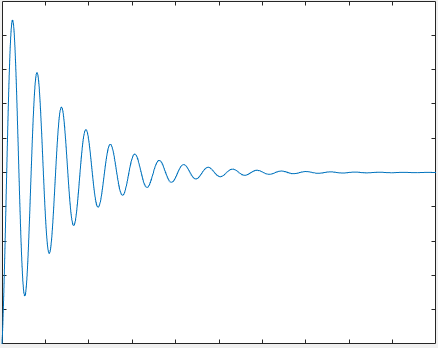
\includegraphics[width=\picturewidth]{pictures/triene.png}
    \caption{Триене}
    \label{fig:friction}
\end{figure}

\noindent
\hrule height 0.1pt
\vskip 0.2cm

Графика на решението на уравнението:
$$
\begin{cases}
    y'' + 5y = 2 \cos(\sqrt{5} t) \\
    y(0) = -1 \\
    y'(0) = 1 \\
\end{cases}
$$

\begin{figure}[H]
    \centering
    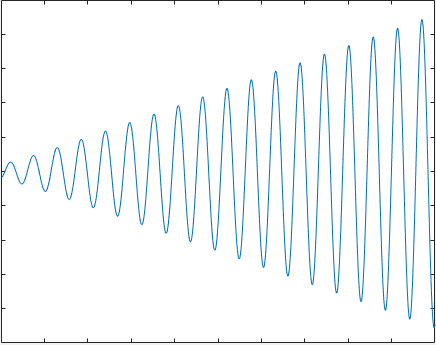
\includegraphics[width=\picturewidth]{pictures/resonans.png}
    \caption{Резонанс}
    \label{fig:resonance}
\end{figure}

\noindent
\hrule height 0.1pt
\vskip 0.2cm

Графика на решението на уравнението:
$$
\begin{cases}
    y'' + 5y = 2 \cos((\sqrt{5} + \epsilon) t) \quad \epsilon > 0 \\
    y(0) = -1 \\
    y'(0) = 1 \\
\end{cases}
$$

\begin{figure}[H]
    \centering
    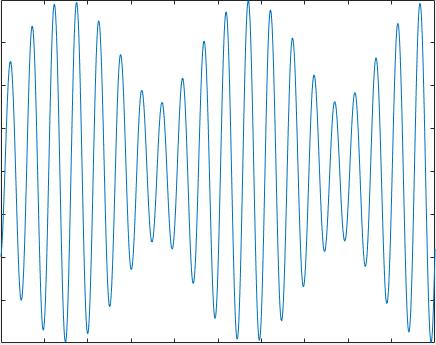
\includegraphics[width=\picturewidth]{pictures/biene.png}
    \caption{Биене}
    \label{fig:beats}
\end{figure}

\noindent
\hrule height 0.1pt
\vskip 0.2cm

\newpage

\subsection{Коментари към получените с MatLab резултати}

\begin{flushleft}
За явлението биене в подточка (3) избраната стойност за $\epsilon$ е $0.3$, защото така се демонстрира явлението
    ясно в дадения интервал $[0, 50]$. \\

\vspace{0.5cm}
В подточка (1) се демонстрира триене, защото стойността на коефициента на загуба на енергия е по-голяма от нула. \\
Ако този коефициент бъде зададен да е 0, то тогава няма да се получава триене, а периодично движение. \\

\vspace{0.2cm}
Графика на решението на уравнението:
$$
\begin{cases}
    y'' + 5y = 0 \\
    y(0) = -1 \\
    y'(0) = 1 \\
\end{cases}
$$

\begin{figure}[H]
    \centering
    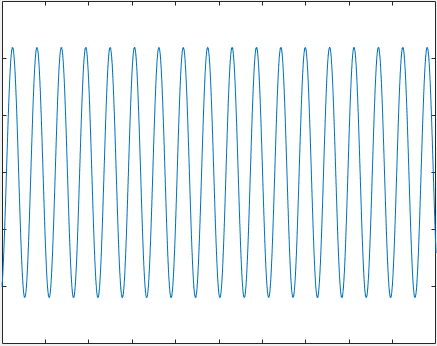
\includegraphics[width=\picturewidth]{pictures/periodichno.png}
    \caption{Периодично движение}
    \label{fig:periodic_movement}
\end{figure}

Аналитичнито решение на това уравнение е аналогично на решението в подточка (1).
\end{flushleft}

\end{document}